\chapter{Srovnání praktické časové náročnosti řešičů} \label{chap:comparison}
\section{Metodika} \label{sec:comparison:metodika}
\subsection{Testovací hry}
Pro porovnání řešičů jsem vytvořil program \benchexe. Ten při běžném použití postupně generuje náhodné Rabinovy hry různých velikostí, nechává je vyřešit vybranými řešiči a zapisuje časy běhů řešičů na jednotlivých hrách do tabulky. Generování her je parametrizováno přes $n$, $k$ a \code{seed} generátoru náhodných čísel \code{rand} použitého jako zdroj náhodnosti.

Pro dané $n$, $k$ a \code{seed} je hra generována po jednotlivých bitech ve vnitřních bitsetech hry. Protože řešič píši pro obecné Rabinovy hry, zvolil jsem pro účely porovnání řešičů pro všechny bity uniformní rozdělení pravděpodobnosti. Tedy mezi dvěma vrcholy vygenerované náhodné hry je hrana s~pravděpodobností $\frac{1}{2}$ a do množiny $g$, resp.~$r$ základní Rabinovy podmínky patří daný vrchol s~pravděpodobností $\frac{1}{2}$.

Velikost testovaných her pokryla rozmezí od triviálních ($n = 0$ nebo $k = 0$) po největší, které bylo lze na použitém počítači vyřešit do řádově jednotek minut.
\subsection{Varianty řešičů}
U každého řešiče jsem testoval zvlášť vyřešení pouhého výherního regionu (\uv{částečné řešení}) a vyřešení výherního regionu s~odpovídající (Adamovou) vyhrávající strategií (\uv{plné řešení}).

U Pitermanova řešiče jsem testoval zvlášť variantu bez store optimalizace a variantu se store optimalizací (viz sekci \ref{subsec:piterman:algoritmus:store}).
\subsection{Testovací prostředí}
Testování jsem provedl na počítači specifikovaném v~tabulce \ref{tab:specifikacepocitace}.
\begin{table}[htbp]
\label{tab:specifikacepocitace}
\caption{Specifikace počítače použitého k~testování}
\begin{center}
\begin{tabular}{|l|l|}
\hline
\multirow{3}{*}{Procesor} & Intel Core2 Duo E7300 \\
 & 2,66 GHz \\
 & 1000 clock ticks za sekundu \\
\hline
Paměť (RAM) & 4,00 GB \\
\hline
Operační systém & Windows 7 Professional 64-bit \\
\hline
\end{tabular}
\end{center}
\end{table}

Čas řešení jsem měřil v~tzv.~clock ticks, tj.~nejmenší časové jednotce měřitelné pomocí standardních knihoven jazyka C++ (v~tomto případě funkcí \code{clock()}). Na použitém počítači odpovídá 1000 clock ticks času jedné sekundy.

Program jsem zkompiloval překladačem G++ z~balíku GCC \cite{GCC}.
\section{Výsledky}
\subsection{MATLABový řešič}
Při testování výkonu jsem zjistil, že MATLABová implementace vrací pro některé hry chybné výsledky. Jako prakticky nepoužitelnou jsem ji proto ze srovnání vynechal. V~digitální příloze jsem zahrnul soubor \path{program/matlab/b2-2-1.mat} s~nejmenší v~MATLABové implementaci chybně řešenou hrou, se kterou jsem se setkal.\footnote{Na správně vyřešených hrách MATLABový řešič vykazoval výrazně horší výsledky, než ostatní řešiče. Pravděpodobně se na tom významnou měrou podepsal použitý převod hry do vstupního formátu MATLABové implementace, který způsobuje kvadratický nárůst velikosti hry vzhledem k~$n$ (viz \ref{sec:matlab:prevod:narustvelikostiinstance}), takže ani v~případě, že by MATLABová impelementace byla korektní, nejspíš by nebylo její porovnání zajímavé.}
\subsection{Pitermanův a Hornův řešič}
V~grafech označuji řešiče z~důvodů prostorových omezení zkrácenými jmény. Vysvětlení těchto jmen najdete v~tabulce \ref{tab:oznaceniresicu}.
\begin{table}[htbp]
\caption{Označení řešičů v~grafech} \label{tab:oznaceniresicu}
\begin{tabular}{l|l}
Popis & Označení \\
\hline
Pitermanův řešič plného řešení bez store optimalizace & PS0 \\
Pitermanův řešič částečného řešení bez store optimalizace & PW0 \\
\emph{Pitermanův řešič plného řešení se store optimalizací} & PS1 \\
Pitermanův řešič částečného řešení se store optimalizací & PW1 \\
\emph{Hornův řešič plného řešení} & HS \\
Hornův řešič částečného řešení & HW
\end{tabular}
\end{table}
\subsubsection{Časy řešení pro $n = 8$}
\begin{figure}[htbp]
\centering
\resizebox{\textwidth}{!}{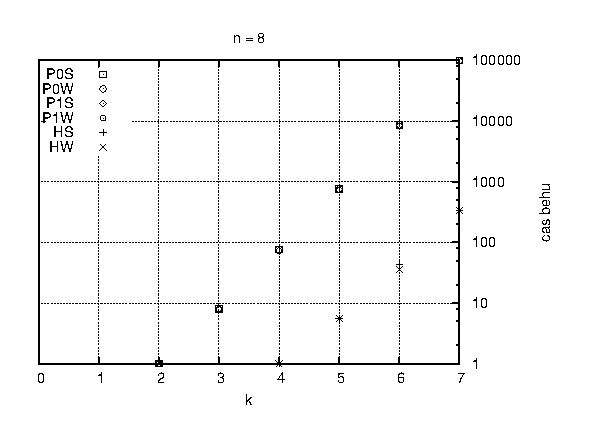
\includegraphics{graph/n8kid-cas}}
\caption{Průměrné časy běhů řešičů na 16 náhodných Rabinových hrách pro $n = 8$}
\label{fig:n8kidcas}
\end{figure}
V~grafu \ref{fig:n8kidcas} jsou zachyceny časy běhů řešičů nad hrami pro fixní $n = 8$ a $k$ pokrývající interval od $0$ do $7$. Pro každé $k$ bylo vygenerováno 16 náhodných her. Vynesené časy běhů jsou průměry přes tyto šestnáctice. Naměřené časy běhů jsou vyneseny v~logaritmické škále.

Fixní $n = 8$ jsem vybral experimentálně jako dostatečně velké pro \uv{zajímavé} chování vzhledem ke $k$.

V~grafu jde vidět, že na použitých hodnotách $n$ a $k$ se jednotlivé varianty Pitermanova řešiče a jednotlivé varianty Hornova řešiče výkonem téměř neliší.\footnote{Jednotlivé varianty řešičů jsou si výsledky tak podobné, že v~grafu téměř splývají. Shluky bodů vynesené výše na ose času běhu patří Pitermanovým řešičům a shluky bodů vynesené níže patří Hornovým řešičům.}

Dále lze pozorovat, že Hornovy řešiče mají proti Pitermanovým výrazně lepší časy běhů.

Absenci hodnot v~levé části grafu přisuzuji nízké rozlišovací schopnosti použitého systému pro měření času -- pro $k \leq 1$ byl na všech řešičích a pro $k \leq 3$ na Hornových řešičích naměřen nulový čas.
\subsubsection{Časy řešení pro $k = 4$}
\begin{figure}[htbp]
\centering
\resizebox{\textwidth}{!}{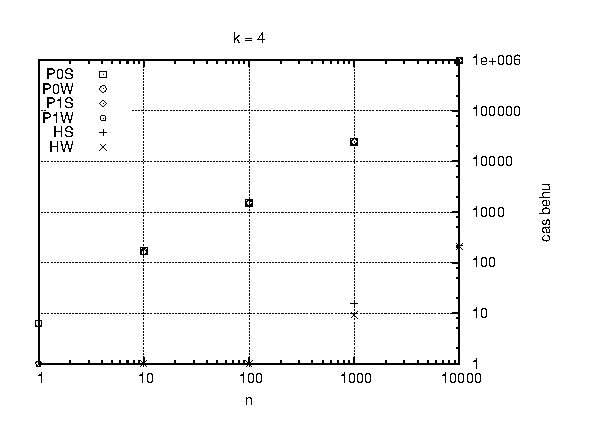
\includegraphics{graph/k4nexp-cas}}
\caption{Průměrné časy běhů řešičů na 16 náhodných Rabinových hrách pro $k = 4$}
\label{fig:k4nexp}
\end{figure}
V~grafu \ref{fig:k4nexp} jsou zachyceny časy běhů řešičů nad hrami pro fixní $k = 4$ a $n$ pokrývající interval od $1$ do $10000$ v~exponenciálních skocích (o základu $10$). Pro každé $n$ bylo vygenerováno 16 náhodných her. Vynesené časy běhů jsou průměry přes tyto šestnáctice. $n$ a naměřené časy běhů jsou vynesené v~logaritmických škálách.

Fixní $k = 4$ jsem vybral experimentálně jako dostatečně velké pro \uv{zajímavé} chování vzhledem k~$n$.

Graf naznačuje podobné relativní vlastnosti řešičů, jako graf \ref{fig:n8kidcas}, zejména podobnost jednotlivých variant řešiců a výrazný rozestup výkonu řešičů ve prospěch Hornova.

Dalo se očekávat, že čas řešení bude velmi podobný pro plné a částečné řešení, protože řešení strategie v~žádném z~použitých algoritmů nezvyšuje asymptotickou složitost. Tento předpoklad analýza potvrdila. Pro další testy jsem se proto rozhodl používat pouze ty varianty řešičů, které řeší plné řešení.

Překvapivým výsledkem je poměrně špatný výkon store-op\-ti\-ma\-li\-zo\-va\-né\-ho Pitermanova řešiče vzhledem k~Pitermanovu řešiči bez optimalizace. Zejména se nezdá, že by vykazoval asymptoticky menší časovou náročnost. Zůstává otázkou, jestli je tato podobnost zapříčiněna neefektivní implementací nebo výběrem testovacích her.